\subsection{Dados}

 O \textit{dataset} utilizado é trata-se da coleta realizadas pela Agência Nacional do Petróleo, Gás Natural e Biocombustível\cite{ANP}.
O \textit{dataset} é a série histórica semanal dos preços e margens de venda de janeiro de 2004 até abril de 2019. Os dados
estão disponíveis para o Brasil inteiro ou segmentados por regiões, por estados ou por 
municípios.

O \textit{dataset} possui os seguintes valores para a semana, a data incial, data final, região, estado,
produto, número de postos pesquisados, unidade de medida, preço médio da revenda,
desvio padrão da revenda, preço mínimo da revenda, preço máximo da revenda,
margem média revenda, coeficiente de variação da revenda, preço médio distribuição,
desvio médio distribuição, preço mínimo da distribuição, preço máximo da distribuição,
margem média distribuição, coeficiente de variação da distribuição, ano e mês.

O gráfico da figura \ref{dataset-graph} mostra os valores do preço médio da revenda ao longo dos anos, é notável a irregularidade nos valores, não sendo possível distinguir se é um erro na anotação ou uma prática do mercado, mas visto a alta recorrência os valores foram considerados como ruídos que possam existir e que não deveriam ser descartados.

A análise limitou-se apenas ao estado de São Paulo e a combustível do tipo gasolina, visto que o objetivo é analisar a viabilidade de utilizar métodos de aprendizado de máquina para a prever o comportamento dos preço.

\begin{figure}[!ht]
\centering
\caption{Gráfico preço médio de revenda de 2004 a 2019  }
\label{dataset-graph}
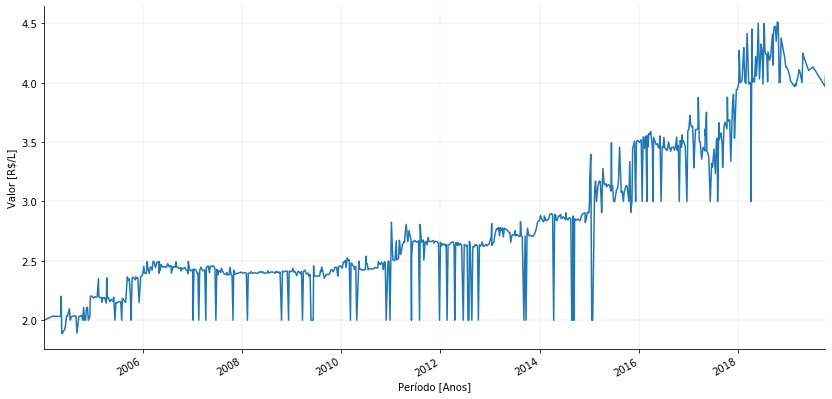
\includegraphics[width=1 \textwidth]{Figuras/precorevenda.png}
\fonte{Próprio autor}
\end{figure}

O gráfico da figura \ref{heatmap} mostra o mapa de calor(\textit{heatmap}) para as \textit{features} não repetidas do \textit{dataset}, ou seja, os valores temporais não são considerados nessa análise. Pela análise do gráfico conclui-se que apenas os coeficientes de variação não são relevantes o bastante para os modelos, os demais valores possuem fortíssima correlação com o preço médio de revenda.

\begin{figure}[!ht]
\centering
\caption{Gráfico de calor da correlação de \textit{features} do \textit{dataset}}
\label{heatmap}
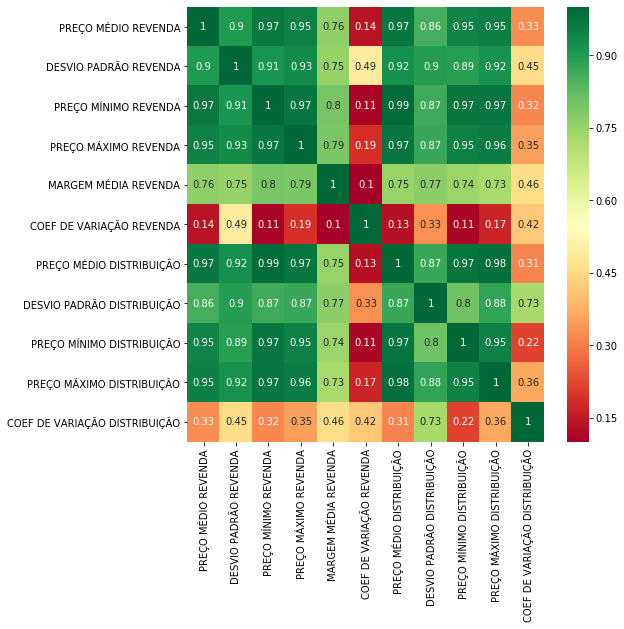
\includegraphics[width=1 \textwidth]{Figuras/heatmap.png}
\fonte{Próprio autor}
\end{figure}

\subsection{Modelos}

Métodos de aprendizado de máquina são em geral aplicados para problemas de regressão(\textit{regression}), classificação(\textit{classification}), redução de ordem(\textit{dimensionally reduction}) e agregação(\textit{clustering}). Previsão de uma série temporal, no caso o preço do combustível, caracteriza-se por um problema de regressão\cite{Eletricity}.

Este trabalho faz uso de alguns dos mais amplamente utilizados  algoritmos de regressão,
são eles \textit{Simple Linear Regression}, \textit{Ridge Regression}, \textit{Support Vector Regression} com \textit{kernel Linear}
e \textit{Radial basis function}\cite{Price}.

Os métodos anteriormente citados foram implementados utilizando a linguagem de programação Python em conjunto com as bibliotecas open sources
\textit{Python Data Analysis Library}(pandas) e \textit{scikit-learn}, a primeira permite o tratamento de dados  como transformação de texto para números e checagem de nível de correlação,
a segunda biblioteca é voltada para aprendizado de máquinas, esta possui os modelos e outras ferramentas utilitárias como
\textit{cross validation}.

Inicialmente separou-se o \textit{dataset} utilizando a biblioteca pandas, limitando-se aos já citados
dados que caracterizariam o problema, data,preço médio de revenda e preço médio de distribuição, também utilizando esta biblioteca foi adicionado a coluna \textit{label} que representa o \textit{target} deste trabalho, o preço de revenda.

Posteriormente, utilizando a biblioteca \textit{scikit-learn} o \textit{dataset} foi dividido em 
teste e treino na proporção 20\% para 80\%. O \textit{dataset} de treinamento foi utilizado para o
treinamento dos modelos. Pós treinamento, a notas de acurácia e os valores
de \textit{cross-validation} foram analisados para checar a precisão do modelo e garantir que não houve \textit{overfitting} durante o treinamento.
